\chapter{Methods}
\label{chap:model}

In this chapter, we firstly present the methodology for our approaches, then describe our aspect-oriented model in detail, begin with an overview of the whole architecture, followed by the explanation of how each of the components work; lastly, we introduce the parameter system used in the model.

\section{Theoretical Basis}
\subsection{K-nearest Neighbors}

KNN is one of the most straightforward supervised algorithms, but effective in dealing some problems, in both classification and regression. KNN does not study anything from training data (therefore it's considered as a lazy learning method)

In classification problem, a new data point's class is derive from k nearest data point from the training set. In general, this label can be calculated by the label of nearest data point \(k=1\) $(weights = uniform)$ or average weight of the nearest points $(weights = distance)$, or a relationship between these weight.

KNN is simple as only two criteria needed: value of \(k\) and the function to calculate distance. KNN does not require any training period because it does not derived any function from training data and only make real-time prediction when evaluating, so this make the algorithm run much faster, especially considering small dataset. New data can be also add anytime without any affection to the algorithm's accuracy.  

Despite lightning performance in small dataset, as the data size enlarges, KNN is not beneficial for both memory and time. The algorithm must remember all the training data for label calculation, so it will become extensively slow as size of dataset grows.

\subsection{Logistics Regression}
LR, in its basic form, uses a logistic function (e.g., sigmoid, tanh) to model a binary dependent variable.
The prediction score of LR is calculated by formula:
\begin{eqnarray*}
f(x) = \theta(\textbf{w}^{T}\textbf{x})
\end{eqnarray*}
where
\begin{description}

\item[] $\theta$: logistics function (e.g., sigmoid, tanh, etc.)
\end{description}
The cost function for LR is defined as:
\begin{eqnarray*}
L = \sum_{D}^{}-ylog(y')-(1-y)log(1-y'))
\end{eqnarray*}
where
\begin{description}
\item[] D: dataset, containing of labeled tuples $(x,y)$
\item[] $y$: the label in a assigned example, which is either be 0 or 1.
\item[] $y'$ is the predicted value, which is between 0 and 1, given features in $x$.
\end{description}

LR is one of the easiest ML algorithms as it is easy to implement, interpret, and very efficient to train. Traning a model with LR doesn't need high computation effort. LR also less prone to overfitting in a low dimensional dataset, and in context of a higher dimensional dataset, regularization can be used to avoid overfitting. Moreover, new data can be updated using stochastic gradient descent (SGD).

But LR also has limitations as it only address linear separable data for non-linear problems transformation is required. Features used for training model should also be carefully extracted otherwise noise will make the probabilistic predictions may be incorrect. LR requires a large dataset and sufficient training examples for all the categories it needs to identify. Lastly, each training tuples must be isolated to all others, because relationship between any of them will make model give more importance to these relative examples.

\subsection{Support Vector Machine}
A SVM model takes data points and outputs the hyperplane (a line in context of two dimensioal dataset) that best separates the classes.

The best hyperplane is the one has largest distance to neares data point of each class. In other words, SVM maximizes the margins from both class.

With nonlinear data, additional dimensions will be required. SVM can classify vectors in multidimensional space. 

\subsection{Naive Bayes}
NB classifier based on applying Bayes' theorem. Bayes' theorem finds out the probability of an event if the occurence another event is probably knows, which is defined as:

\begin{eqnarray*}
 \Pr(A|B)=\frac{\Pr(B|A)\Pr(A)}{\Pr(B|A)\Pr(A)+\Pr(B|\neg A)\Pr(\neg A)}f(x)
\end{eqnarray*}
where A and B are events.

NB classifiers assumed all the features are independent and equally contributed to final result. Probability of feature $y$ given a set of $X$ features as ${x_{1}, x_{2}, ..., x_{n}}$ is calculated by formula: 

\begin{eqnarray*}
P(y|x_{1}, x_{2}, ..., x_{n}) = \frac{P(x_{1}|y)P(x_{2}|y)...P(x_{n}|y)P(y)}{P(x_{1})P(x_{2})...P(x_{n})}
\end{eqnarray*}

We find the probability of all possible values of class $y$ and choose the maximum, which can be expressed as:

\begin{equation}
    y = argmax_{y}P(y)\prod_{i=1}^{n}P(x_{i}|y)
\end{equation}

Although completely independent features are barely exist, in practical terms NB is widely used since it's highly scalable, time-saving and suitable for categorical input variables.

\subsection{Decision Tree}
A decision tree is used to represent decisions and decision-making process. The tree can be explained as the leaves, which is final outcome, and the decision node, which is the place data splits.

For classification purpose, the outcomes (or leaves) are corresponding to features, which is selected throughout the tree. Begin with the root, or the starting node, we find out the best decision (e.g., best attribute) by applying selection measures (Information Gain, Gini Index, etc.) in the dataset, then divide dataset into subsets and recursively perform the process until the nodes can not be further divided. The leaf nodes now is the final outcome, and the total process make out the model.

\subsection{Random Forest}
RF is the combination of multiple DT that opearate as an ensemble, which results in more reliable and stable prediction. Each DT finds out a class prediction, and the most chosen becomes the total model's prediction. As those DTs are relatively independent, RF is protected from individual DT's error (unless all the DTs are wrong in the same way).

RF works well with categorical variables. Missing or imbalanced values can be handled easily. Noise or new data point also not a problem as it can only affect some of DTs but not to entire forest.

\subsection{Convolutional Neural Network}
CNN is a popular Deep Learning model. A typical CNN consists of a set of basic layers including: convolution layer with kernels, pooling layer, fully connected layer, which are linked together in a certain order.

Convolution is the first class to extract the features from the input sentence. Convolution maintains relationship between words by exploring sentence feature by using small segments of input data. It is a mathematical operation that takes two inputs such as a matrix of words and filter of kernels.

The maxpooling layer will reduce the number of parameters when the word count is too large. Spatial aggregation is also known as sub-sampling, which reduces the dimensionals of each map but retains important information.

The last layer flattens its matrix into vector and brings it to a fully connected layer like a neural network, which combines the features together to create a model. 

Finally, we have a activation function like softmax or sigmoid to to classify with probability value from 0 to 1.




% -----------------------------------------------------------------
% Introduction of the chapter
% -------------------------------------------------------------------

\section{Model overview}
\label{sec:overview}
\begin{figure}[h]
	\centering
	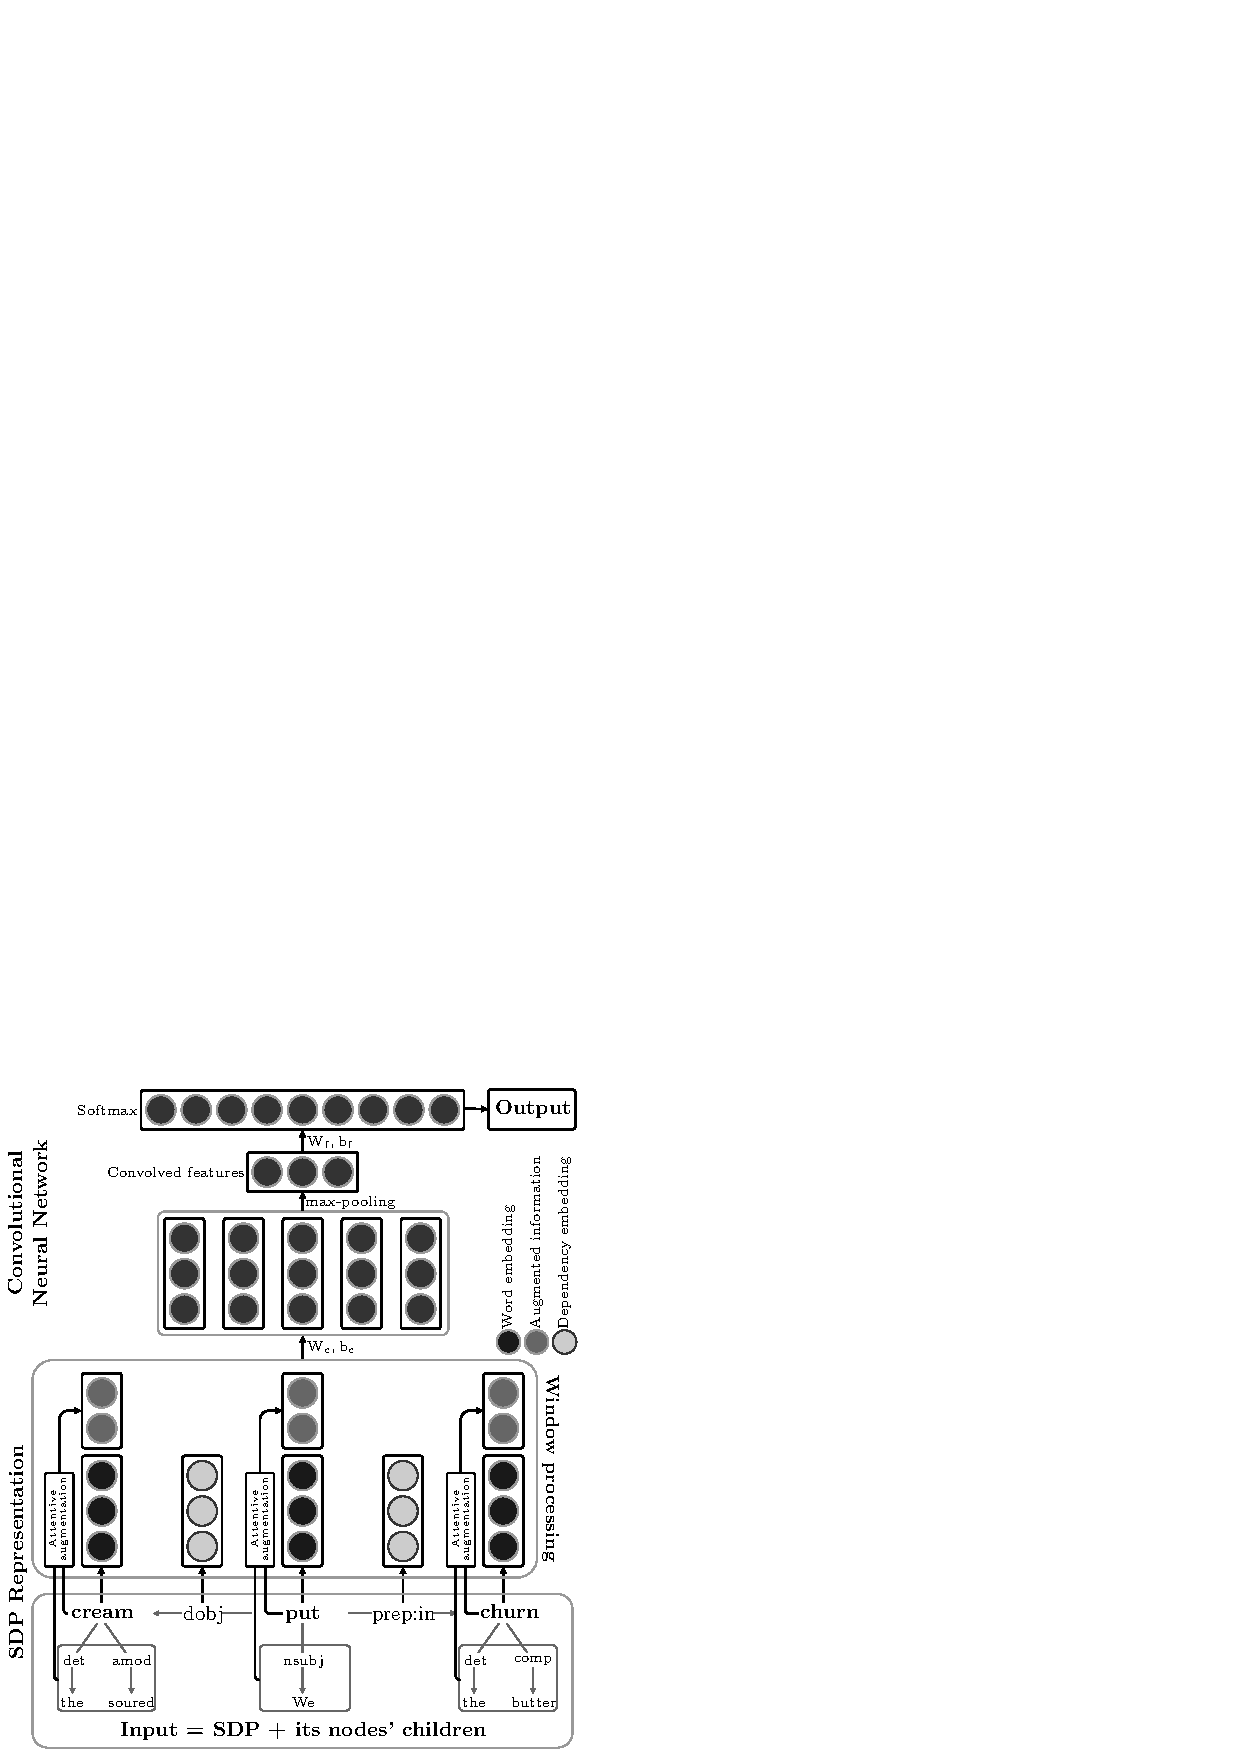
\includegraphics[width=\linewidth]{Chapter3/Figs/model.pdf}
	\caption{The aspect and sentiment analysis pipeline}
	\label{fig:model1}
\end{figure}
The main objective of our model is to address the second sub-task of the ABSA problem as it must be able to perform the aspect polarity task. In this case, the system should identify which of two polarity labels - positive or negative could be assigned with the corresponding aspect. Figure \ref{fig:model1} shows the position of our problem in the opinion mining overall architecture. In which aspect recognition is considered as the preceding problem of sentiment classification and is outside the scope of this study. In this report, we assume that aspect recognition is completed before.

Our aspect-oriented sentiment analysis model consists of four main phases, illustrated in Figure~\ref{fig:model2}: reprocessing, locating, representation and classification. The first phase helps cleaning and preparing data for classification, the second one applies word-window method to find out the words which has a high ability to decide which sentimental status the aspects are. Following to that, we tested different ways to represent words with a view to extract meaningful features from data. Finally, the last phase is our application of multiple classifiers, including both classic ones like SVM, Random Forest, etc. and modern one as Deep Learning, which will be all described within this section.

\begin{figure}[h]
	\centering
	\includegraphics[width=\linewidth]{Chapter3/Figs/model2.pdf}
	\caption{Implementation steps for a single aspect}
	\label{fig:model2}
\end{figure}

\section{Preprocessing}
\label{sec:preprocessing}
Preprocessing is one of the key steps in every natural language processing problem as it transforms data into usable one which machine can easily interprete. Since the characteristics of the input data are raw text collected from websites, the input text (from the dataset contains the specific aspect that we have gathered and processed in Chapter~\ref{chap:dataset-construction} above) can have noise which can harmful to machine learning performance such as special characters, spelling mistakes, spacing errors, etc. To standardize the data and reduce the amount of noise, preprocessing process is applied according to the following steps:

\begin{itemize}
  \item \textbf{Step 1:} Special characters (including punctuations) were completely removed.
  \item \textbf{Step 2:} Trim unnecessary spaces made by spacing errors.
  \item \textbf{Step 3:} Lowercase all characters.
  \item \textbf{Step 4:} Transfer acronyms to the full form of them and translated from context.
  %\item \textbf{Step 5:} Delete stop words. A stop word is a commonly used word that the machine should avoid learning to save space and time processing. They do not act as meaningful criteria in our approach, so basically all of them were removed. However, some of the normal stop words may determine the sentiment, so we have to take an extra step manually to keep this kind of stop words.
  \item \textbf{Step 5:} Word tokenization. Tokenization is essentially splitting a phrase, sentence, paragraph, or an entire text document into smaller units called tokens, such as individual words or terms. By tokenization, the meaning of the text can be interpret easier by some analysing methods such as count the number of words appeared, the frequency of the word, and so on.
\end{itemize}


\begin{table}[]
\begin{otherlanguage}{vietnamese}
\begin{tabular}{|c|>{\raggedright\arraybackslash}m{13 cm}|}
\hline
\textbf{Input}  & \textbf{Bỉm mềm , chất lượng tốt , hút dc nhiều nhưng \(  \) giao hàng khá chậm.} \\ \hline
\textbf{Step 1} & Bỉm mềm \(  \) chất lượng tốt\(  \) hút dc nhiều nhưng \(  \) giao hàng khá chậm                     \\ \hline
\textbf{Step 2} & Bỉm mềm chất lượng tốt hút dc nhiều nhưng giao hàng khá chậm                        \\ \hline
\textbf{Step 3} & bỉm mềm chất lượng tốt hút dc nhiều nhưng giao hàng khá chậm                        \\ \hline
\textbf{Step 4} & bỉm mềm chất lượng tốt hút được nhiều nhưng giao hàng khá chậm                      \\ \hline
%\textbf{Step 5} & bỉm mềm chất lượng tốt hút nhiều giao hàng chậm                                     \\ \hline
\textbf{Step 5} & \textbf{bỉm mềm chất\_lượng tốt hút nhiều giao\_hàng chậm}                          \\ \hline
\end{tabular}
\end{otherlanguage}
\caption{Step-by-step preprocessing illustration}
\label{tab:my-table}
\end{table}

VnCoreNLP (Vu et al., 2018 \cite{vu-etal-2018-vncorenlp}) is used for all pre-processing steps.

\section{Locating}
\label{sec:locating}
\subsection{Chi-Squared Test for Feature Selection}
\label{subsec:chi2}
\paragraph{}
In statistics, the Chi-squared test is used to determine whether two categorical variables independent or related. In feature selection, the two variables are the observations of the feature and the occurrence of the class. The outcome of the test is a test statistic that has a chi-squared distribution and can be clarified or fail to reject the assumption or null hypothesis \(H_{0}\) that the observed and expected frequencies are equal.

Given a document \(D\), we estimate the (\(\chi^{2}\)) value and rank them by their score:
\begin{eqnarray*}
\chi ^{2}= \sum_{t=1}^{}\sum_{c=1}^{}\frac{(O_{t,c}-E_{t,c})^{2}}{E_{t,c}} = N\sum_{t,c}^{}p_{t}p_{c}\left(\frac{(O_{t,c}/N)-p_{t}p_{c}}{p_{t}p_{c}}\right)^{2} \\
\end{eqnarray*}
where
\begin{description}
\item[] \(\chi^{2}\) = Pearson's cumulative test statistic, which asymptotically approaches a \(\chi^{2}\) distribution.
\item[] \(O_{t,c}\) = the number of observations of type \(t\) in class \(c\).
\item[]\(N\) = total number of observations.
\item[]\(E_{t,c} = Np_{t,c}\) = the expected (theoretical) count of type \(t\) in class \(c\), asserted by the null hypothesis that the fraction of type \(t\) in class \(c\) in the population is \(p_{t,c}\)
\end{description}

For each feature, a corresponding high \(\chi^{2}\) score indicates that the null hypothesis of independence (meaning the document class has no impact over the term's frequency) should be dismissed and the occurrence of the term and class are dependent, therefore we should select the feature for classification. In other words, using this method remove the feature that are most likely autonomous of class and consequently unessential for classification.

We use Scikit-learn (Pedregosa et al., 2011 \cite{scikit-learn}) as it provide multiple feature selection methods, including Chi-Squared Test. Scikit-learn gives a \emph{SelectKBest} class that can be used with various statistical tests. It will rank the features with the statistical test that we've determined (Chi-Squared Test in detail) and select the top \(k\) performing ones (implying that these terms is viewed as more relevant to the task than the others). These top performing features will be used for locating and one of the representation method that we will described below.

\subsection{Word-Window Locating}
\begin{figure}[h]
	\centering
	\includegraphics[width=\linewidth]{Chapter3/Figs/window.pdf}
	\caption{Word-Window Locating process}
	\label{fig:wwl}
\end{figure}

We use chi-squared rank as calculated above to weight the words in the comment, with a view to select out which word play the important role on determine aspect's sentiment.

Given a sentence as a set of word \(W = \{w_{0}, w_{1}, w_{2}, ..., w_{n}\}\) and a set of class \(C = \{c_{0}, c_{1}, c_{2}, ..., c_{m}\}\), we simply define score \(s_{i,j}\) as \(\chi^{2}\) score of the word \(w_{i}\) in class \(c_{j}\). For each aspect \(c_{j}\) , we choose a threshold \(s_{c_{j}}\), and ignore all the words which have lower score than that threshold. If the sentence has no word with score higher than threshold, the word with highest score will be selected.
Based on calculation above, we take out 3 words before and after the high-score word \(w_{i}\). This combination, or \emph{window}, can be illustrated as: \(\{w_{i-3}, w_{i-2}, w_{i-1}, w_{i}, w_{i+1}, w_{i+2}, w_{i+3}\}\)

The results collected is helpful for classifier as WWL removed the non-related words of each aspect and its sentiment; therefore, only relevant words extracted to put in learning model.

\section{Representation}
\subsection{One Hot encoding}
Every word which are part of the text data are written in the form of vectors, constituting only of 1 and 0 (1 if word in vocabulary else 0). Although it does not highlight the importance of words in sentiment classification, but it has yielded quite surprising results. Further information will be provided in Section~\ref{sec:experiment-result}.

% Description in more detail will be proposed in Chapter~\ref{chap:experiments}.

% \begin{table}[]
% \centering
% \begin{tabular}{|c|c|c|c|c|c|c|}
% \hline
% \multicolumn{1}{|l|}{} & \textit{\textbf{price}} & \textit{\textbf{service}} & \textit{\textbf{safety}} & \textit{\textbf{quality}} & \textit{\textbf{delivery}} & \textit{\textbf{authenticity}} \\ \hline
% \textbf{LR}            & 0.89177                 & 0.92404                   & 0.96264                  & 0.94759                   & 0.93300                    & 0.94307                        \\ \hline
% \textbf{RF}            & 0.90335                 & 0.94085                   & 0.95587                  & 0.95715                   & 0.93752                    & 0.95852                        \\ \hline
% \textbf{DT}            & 0.87578                 & 0.93300                   & 0.94412                  & 0.94813                   & 0.91102                    & 0.95124                        \\ \hline
% \textbf{NB}            & 0.69943                 & 0.85465                   & 0.88525                  & 0.78723                   & 0.78005                    & 0.79697                        \\ \hline
% \textbf{KNN}           & 0.86871                 & 0.92856                   & 0.94153                  & 0.94271                   & 0.89603                    & 0.93361                        \\ \hline
% \textbf{SVM}           & 0.81661                 & 0.92477                   & 0.93397                  & 0.94200                   & 0.89992                    & 0.93584                        \\ \hline
% \end{tabular}
% \caption{Average F1 Score of 5-fold Cross Validation}
% \label{table:chi2}
% \end{table}

\subsection{Chi-Squared}
We use word-level \(\chi^{2}\) as calculated above to weight the words in the vocabulary, and use that vocabulary to represent data. Then we proceed to filter each aspect's vocabulary manually to reduce dimensions used for classfiers. The results using this data representation method shown in Section~\ref{sec:experiment-result}.

\subsection{Word Embedding using PhoBERT}
\label{subsec:word-embedding}
\paragraph{BERT}
BERT (Bidirectional Encoder Representations from Transformers) is understood as a pre-trained model, which learns vectors that represent two dimensions of words while models such as Word2vec, fastText find a vector that represents each word based on a large set of materials, so it does not represent the diversity of context. BERT has succeeded in improving recent work in finding representatives of words in digital spaces (spaces that computers can understand) through its context. 

Transformer is an attention mechanism that learns the correlation between words (or part of a word) in a text. Transformer consists of two main parts: Encoder and Decoder, encoder that reads input data and decoder makes predictions. In this sitution, BERT uses only Encoder.

BERT is used to support other problems in the field of natural language processing such as emotional classification, amantic analysis, spam filtering, news classification, etc. Our proposed work use BERT for the problem of sentment classification.

\paragraph{PhoBERT}
Pre-trained PhoBERT models are the state-of-the-art language models for Vietnamese (\citeauthor{phobert}~ \cite{phobert}). PhoBERT uses VnCoreNLP to separate words for input data before passing encoder.

PhoBERT output consists of 2 layers: the first one is the last hidden layer created by token embedding, sentences embedding, transformer positional embedding into a 3D vector, while the second is the layer that has been pooling into a 2D vector.

In each string of words after using PhoBERT, we have two ways of expressing the word and sentence level:
\begin{itemize}
    \item Represented by word level: each word will be represented as a 768-dimensional vector, so in total a \(n*\)768 matrix will represent a sentence.
    \item Represented by sentence level: the whole sentence is also represented by a 768-dimensional vector.
\end{itemize}

Typically, a sentence after being represented by the matrix bar will be spread through the convolution layer + nonlinear layer first (RELU), after which the calculated values will spread through the pooling layer, multiple kernels.

Specifically, the word vectors from $w_{i}$ to $w_{i+j-1}$ as $[w_{i}, w_{i+1}, w_{i+2},...,w_{i+j-1}]$ will be combine to represent one feature. Afterwards, a filter is applied to the specific k-word vector (in the proposed work we use k = 2, 3 and 4) to captured most useful features for sentiment detection. 

Feature $c_{i}$ is generated from a nonlinear activation function (hyperbolic tangent or ReLU)
\begin{equation}
    c_{i} = f(F(w_{i,i+k}^{}+b)
\end{equation}
where $b$ is a bias, a vector performs as a additional function to the input.

We will get 1 characteristic matrix for a specific feature:
$c = [c_{1}, c_{2}, c_{3},...,c_{h}]$
Then, maxpooling (take out the maximum characteristic $c_{i}$ among the matrix) is applied to choose the most important features. The reason for choosing the highest $c$ is because the input will inevitably map to a fixed output size so that it is fully connected, the input size is reduced but still maintains important properties. 

The convolution filer number is certain with different width and slips across the entire matrix to get all the properties.


